%% This is an example first chapter.  You should put chapter/appendix that you
%% write into a separate file, and add a line \include{yourfilename} to
%% main.tex, where `yourfilename.tex' is the name of the chapter/appendix file.
%% You can process specific files by typing their names in at the 
%% \files=
%% prompt when you run the file main.tex through LaTeX.
\chapter{Introduction}\label{intro-ch}

A number of applications require a domain expert to visually inspect and
process a stream of incoming data. The problem with manual inspection is the
inability to scale as datasets grow exponentially \cite{exp-growth}. As the
dataset grows, it becomes difficult to visualize interactively \cite{immens}.
In this thesis we focus on medical data, where doctors have to analyze a
patient's data and extract relevant information for treatment. Specifically, we
focus on electroencephalogram (EEG) readings, a test which used to detect
abnormalities related to the electrical activity of the brain. \\

Today, doctors store large amounts of patient data that they cannot analyze
because they lack tools to efficiently view datasets at scale. To address this
issue, we have designed and implemented Pinky, a system for processing large
amounts of EEG data, allowing near real-time interactive analysis.


\section{Pinky}

Pinky is a doctor's newest tool for analyzing the brain, see
Figure~\ref{fig:pinky-and-the-brain}. Working with a team of researchers at
Massachusetts General Hospital (MGH), we have designed and implemented the
system to handle the fast growing corpus of collected EEG data. This end-to-end
system handles the storage, processing, and visualization of EEG data. The
goal of the system is to provide a scalable architecture for concurrent
analysis of patient records with near real-time interactivity. Each layer of
the system is optimized for use and evaluated across hundreds of gigabytes of
patient data. \\

\begin{figure}[h]
\begin{center}
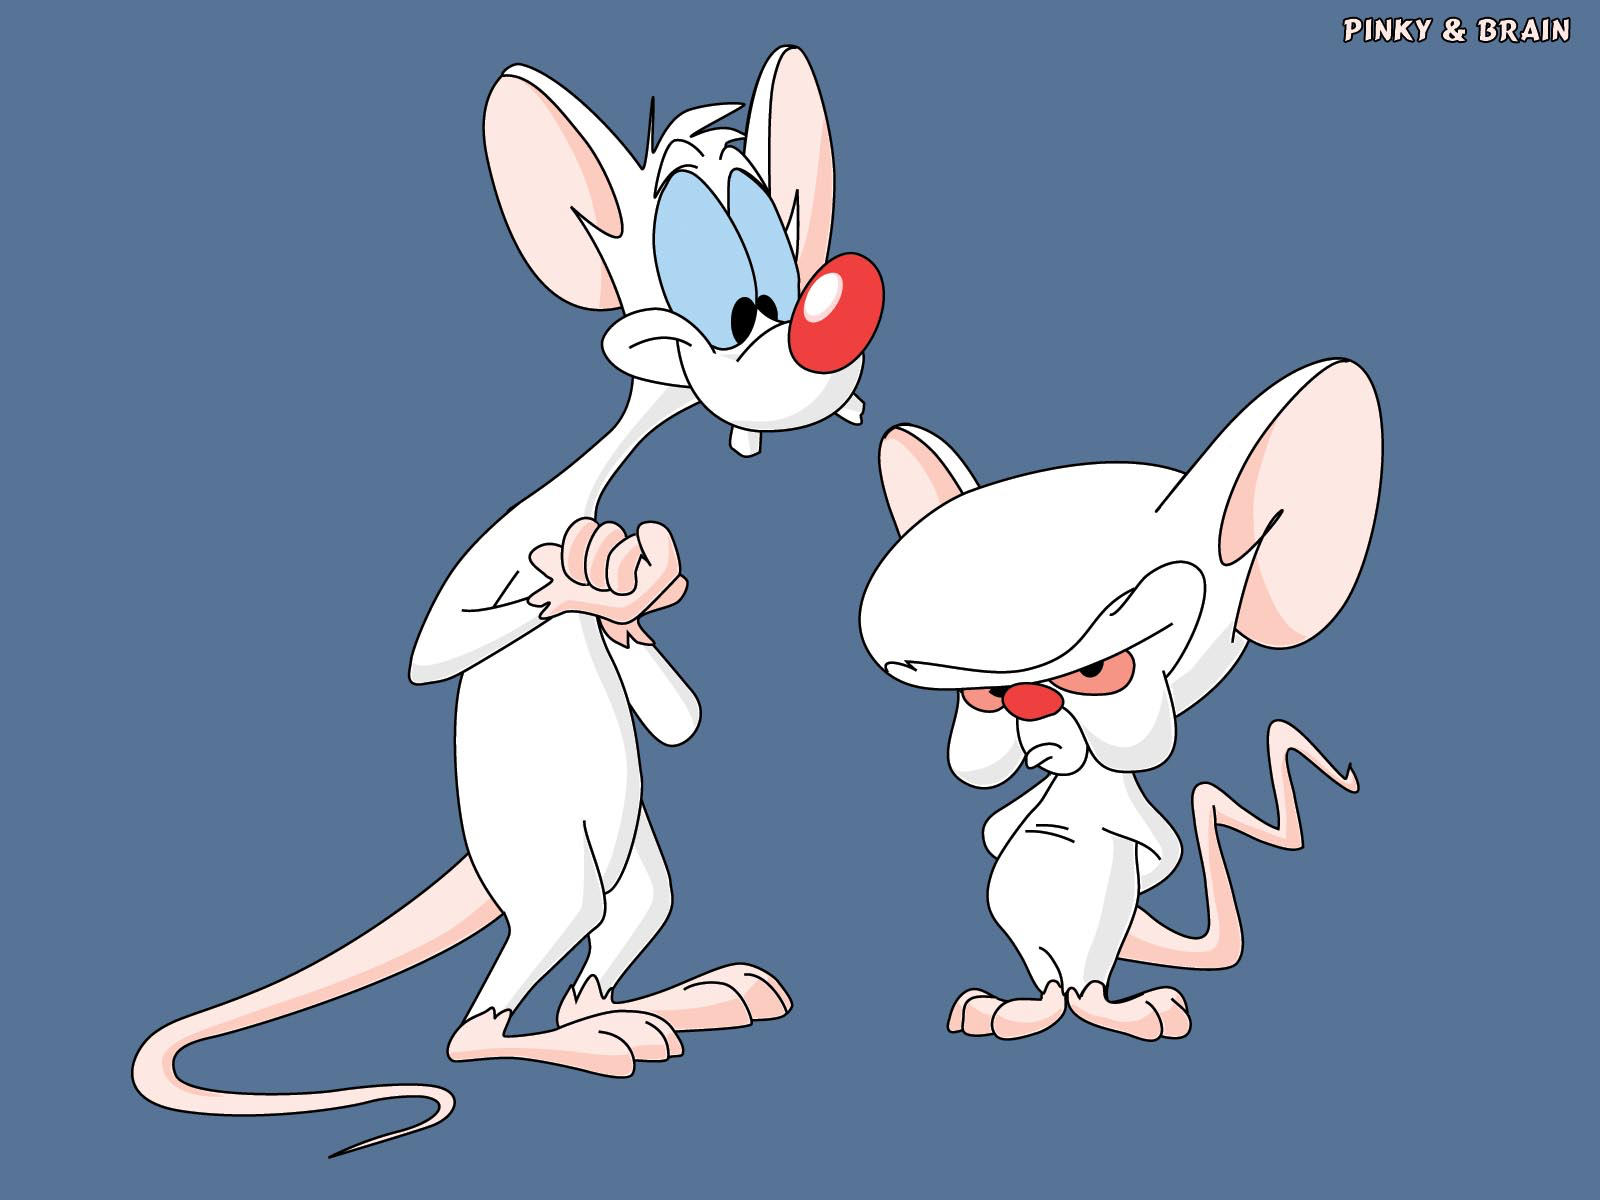
\includegraphics[scale=0.5]{./img/pinky-and-the-brain.png}
\caption{Etymology of Pinky's name.}
\label{fig:pinky-and-the-brain}
\end{center}
\end{figure}

\section{Overview of EEG Analysis}\label{intro-ch:eeg-overview}

A seizure is a transient aberration in the brain's electrical activity. People
with the central nervous system disorder epilepsy suffer from recurrent
seizures, often happening suddenly and at unpredictable times. A seizure can
vary from a lapse of attention to a whole-body convulsion. Frequent seizures
are dangerous, as they can increase risk of sustaining physical injuries and
can even result in death \cite{eeg-ml}. \\

One method for detecting the onset of epileptic seizures is the analysis of
scalp EEG data, a non-invasive measure of the brain's electrical activity.
Continuous EEG (cEEG) data is typically recorded using 19 silver/silver
chloride electrodes, affixed to the scalp \cite{ceeg-1}.
Figure~\ref{fig:electrodes} shows a drawing of the placement of sensors on a
patient's scalp. \\

\begin{figure}[h]
\begin{center}
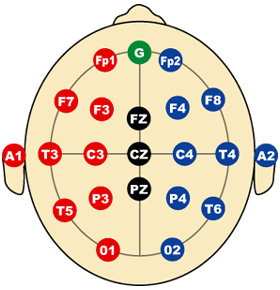
\includegraphics[scale=0.5]{./img/electrodes.png}
\caption{EEG electrode placement on a patient's scalp.}
\label{fig:electrodes}
\end{center}
\end{figure}

Trained individuals, such as attending physicians, epilepsy/neurophysiology
fellows, or registered EEG technicians (encephalographers), review and screen
EEG recordings, which typically take place over a continuous 24-hour period
\cite{ceeg-3}. Unlike traditional epilepsy monitoring units which focus on
provoking and capturing seizures, the goal of cEEG studies is to efficiently
identify future seizures and prevent them. This leads to an increase in the
number of cEEG recordings for preventative measures. Intensive care unit
centers are subsequently overwhelmed with the analysis of the growing dataset
due to the small number of available trained individuals. Methods to screen
long EEG recordings without sacrificing accuracy are necessary to be able to
efficiently process this data. \\

Typically, EEGs displays show no more than 10 to 15 seconds of data per screen
of raw voltage readings and requires an analyst to simultaneously inspect
multiple channels. In contrast, a compressed spectral array \cite{csa} or
spectrogram display may show 2 to 8 hours of data on a single color map
\cite{ceeg-3}. This allows analysts to quickly screen long periods of EEG data,
determining which segments, if any, require direct review of the raw data.
Spectrogram review reduces cEEG review time by $78\%$ \cite{ceeg-2}, with
minimal loss of sensitivity compared with conventional review. For these
reasons, we focus on building a tool to rapidly analyze spectrogram data. \\

\begin{figure}[h]
\begin{center}
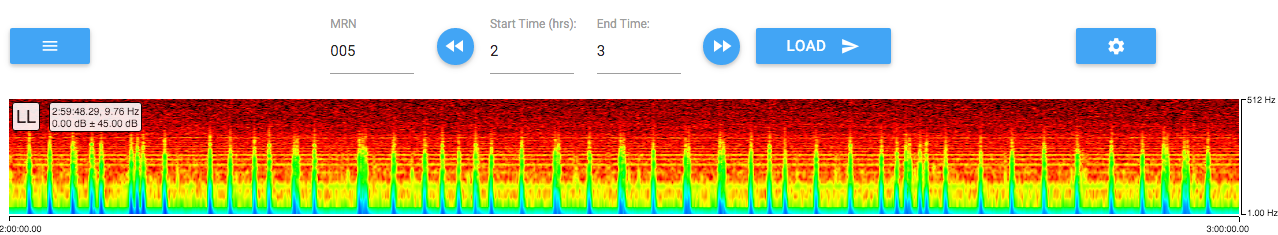
\includegraphics[scale=0.35]{./img/eeg-view.png}
\caption{Spectrogram for one hour window of EEG data of the \c{LL} region of
  the brain.}
\label{fig:eeg-view}
\end{center}
\end{figure}

Spectrograms are the most widely used compressed data format for EEG data
\cite{ceeg-1}. A spectrogram consists of three-dimensional plots with time on
the x-axis, frequency on the y-axis, and EEG power on the z-axis.
Figure~\ref{fig:eeg-view} shows an example of rendered spectrogram data. An
analyst typically views four spectrograms concurrently, mapped to different
regions of the brain. Each region is formed by using multiple EEG channels
where an EEG channel is the difference between voltages measured at two
electrodes. This captures the summed potential of millions of neurons
\cite{eeg-ml}.  Figure~\ref{fig:electrodes} shows the electrode placement on
the patient's scalp, yielding four regions for analysis: left lateral power,
\c{LL}, (Fp1-F7, F7-T3, T3-T5, T5-O1), left parasagittal power, \c{LP},
(Fp1-F3, F3-C3, C3-P3, P3-O1), right lateral power, \c{RL}, (Fp2-F8, F8-T4,
T4-T6, T6-O2), right parasagittal power, \c{RP}, (Fp1-F4, F3-C4, C4-P4, P4-O2).
\\

Data from a single patient can vary in size from tens to hundreds of gigabytes
and the number of EEG tests performed each year is estimated to be between 10
and 25 million \cite{eeg-scale}. As this corpus of data collected at the ICU
continues to grow, efficient mechanisms to store and visualize this data at
scale are key for analysts to quickly view patient screenings. Pinky aims to
provide this for analysts by giving them a simple yet powerful interface to
view spectrogram data.

\section{System Architecture}

Pinky is comprised of three coupled layers which handle storage, computation
and visualization. Figure~\ref{fig:system-architecture} shows the overall
architecture of the system.

\begin{figure}[h]
\begin{center}
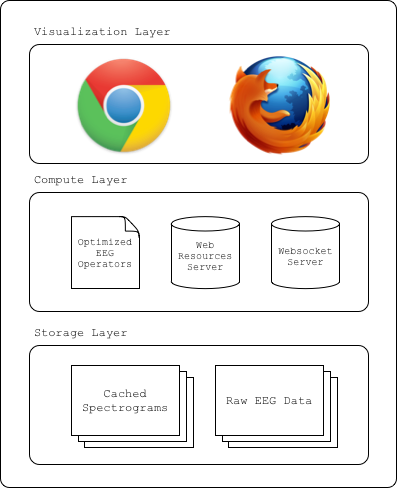
\includegraphics[scale=0.75]{./img/system-architecture.png}
\caption{Pinky system architecture.}
\label{fig:system-architecture}
\end{center}
\end{figure}

\subsection{Storage Layer}

The storage layer, discussed in detail in Chapter~\ref{storage-ch}, is
responsible for storing raw EEG patient data and the calculated spectrogram.
This datastore must optimize both reads and writes of array based data for
multidimensional arrays on the order of tens to hundreds of gigabytes.

\subsection{Compute Layer}

The compute layer, discussed in detail in Chapter~\ref{compute-ch}, is an
extensible module which handles the algorithms to calculate the spectrogram and
other EEG related calculations. As we discuss in
Section~\ref{discuss-ch:future-work}, there are a number of extensions the
project can take, thus it is important that an interested developer can easily
add functionality to this layer. In addition, the compute layer contains two
servers. One server interfaces with the optimized EEG algorithms and the
storage layer to serve array based data. The second server is a lightweight
server for the web resources of the visualization layer.

\subsection{Visualization Layer}

The visualization layer, discussed in detail in Chapter~\ref{viz-ch}, is a browser
based module that renders the data to the client. The interface allows users to
query based on a patient's id (medical record number, \c{mrn}) and view a spectrogram
for a given time interval. An analyst may smoothly pan and zoom throughout the dataset.

\subsection{Visgoth System}

Since enabling interactivity is an important design criteria, we have designed
and built an optimization module for browser based visualizations named
Visgoth. The system uses profiling information from the client and server to
suggest an adaptive scaling of the visualizations served in order to keep
latency consistent, regardless of a client's hardware or network bandwidth. We
discuss Visgoth in detail in Chapter~\ref{visgoth-ch}.

\section{Usage}

The project code base is available publicly on Github \cite{github} at
\url{https://github.com/joshblum/eeg-toolkit}, with documentation for
installing the project for development. In addition, we have created Docker
\cite{docker} images that can easily be installed for production use. Armed
with a dataset, any curious doctor is able to install the images and load the
data for analysis. The docker images are available for public use on DockerHub:
\url{https://hub.docker.com/r/joshblum/eeg-toolkit-webapp} and
\url{https://hub.docker.com/r/joshblum/eeg-toolkit-toolkit}. The Github project
contains specific installation instructions.

\section{Contributions}

Pinky makes the following contributions:

\begin{itemize}

  \item Implements an abstraction for array based storage systems.

  \item Implements three different backends which adhere to the abstraction.

  \item Evaluates the different backends for varying input ranges and
    workloads.

  \item Implements optimized algorithms for analyzing EEG data.

  \item Provides an extensible framework for accessing array based data and
    visualizing it in the browser.

  \item Implements scalable in-browser visualizations using the client's GPU.

  \item Implements a new system, Visgoth, for reducing latency for browser
    based visualizations.

\end{itemize}

These contributions enable doctors and medical expert analysts to interactively
analyze EEG data at scale.

